\documentclass[12pt, letterpaper]{article}
\usepackage[colorlinks]{hyperref}
\usepackage[utf8]{inputenc}
\usepackage{graphicx}
\usepackage[font=small,skip=-1pt]{caption}
\usepackage{subcaption}
\usepackage{amsmath}
\usepackage{placeins}
\graphicspath{ {./plots/} }

\title{Analysis Report on Inspecting MQTT}
\author{Liyao Tang - u6142160}
\date{ \today}

\begin{document}
\begin{titlepage}
	\maketitle
\end{titlepage}

\section{Analysis on Handshakes under Different QoS}

Figure \ref{fig:handshake_snap_shot} shows the required screenshots. QoS defines the handshake of the sending and receiving of one message between the sender and receiver, which both can be either broker or devices. For each QoS level, an explanation of its handshake are given as follow.
\begin{enumerate}

	\item QoS = 0
	
	The application message is delivered according to the best efforts of the underlying TCP/IP network and sender would discard the application message once sent out. 
	
	Hence, the application message will arrive at receiver at most once.
	
	\item QoS = 1
	
	After application message sent, sender waits for an acknowledgement (PUBACK or Publish Ack) to make sure the application message is received. To match PUBACK with corresponding application message, each application message at this QoS level has an ID. After PUBACK received, application message can be safely discarded.
	
	After a predefined time without returning PUBACK for the application message, sender will re-send application message with its DUP flag set, meaning this is duplicate. 
	
	Hence, the application message will arrive at receiver at least once.
	
	\item QoS = 2
	
	After application message sent, sender waits for an acknowledgement (PUBREC or Publish Received) to ensure application message is received and then responds with a further acknowledgement (PUBREL or Publish Release) to acknowledge that it knows application message is received. Afterwards, sender still needs to wait for one more acknowledgement (PUBCOMP or Publish Complete) from receiver so that sender is sure that receiver has received the PUBREL. Finally, the application message can be safely discarded.
	
	After a predefined time without the expecting message, the protocol (either sender or receiver) will retry from the last unacknowledged message.
	
	Hence, the application message will arrive at receiver exactly once.
	
\end{enumerate}

As listed above, those assisting messages that is not compulsory for application to meet its specification can transmit on QoS level 0; whereas those key messages, which may results in deviation from the specification if not received, should transmit under QoS level 1; while some important messages whose not only payload but also occurrence matter should transmit under QoS level 2 because duplicate messages are not applicable under this circumstance.

\begin{figure}
	\centering
	\begin{subfigure}[t]{0.77\textwidth}
		\centering
		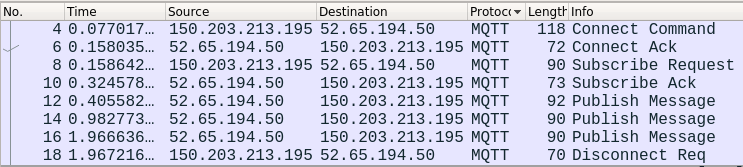
\includegraphics[width=\textwidth]{wire_shark/handshake-q0}
		\caption{QoS = 0}
	\end{subfigure}
	
	\begin{subfigure}[t]{0.77\textwidth}
		\centering
		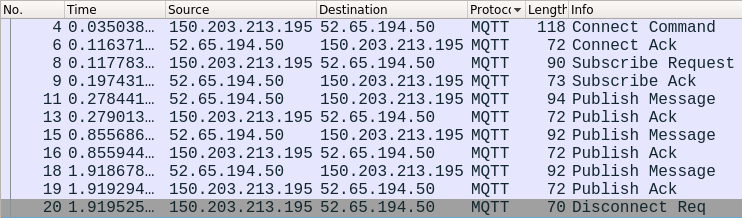
\includegraphics[width=\textwidth]{wire_shark/handshake-q1}
		\caption{QoS = 1}
	\end{subfigure}
	
	\begin{subfigure}[t]{0.77\textwidth}
		\centering
		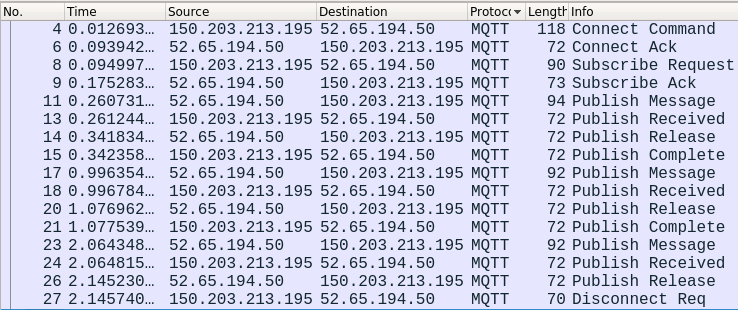
\includegraphics[width=\textwidth]{wire_shark/handshake-q2}
		\caption{QoS = 2}
	\end{subfigure}

	\caption{Figures of MQTT handshake under different QoS. The client disconnects the broker after receives three messages.}
	\label{fig:handshake_snap_shot}
\end{figure}

\section{Statistical Analysis for Each QoS Level}

\subsection{Collecting Statistics}

\subsubsection{Code Structure and Explanation}

The code is written in python3.6.4, using MQTT library and several other standard python libraries, including OptionParser, time, sys and gc.

The code takes two compulsory command line parameters, explained as follow:
\begin{itemize}
	\item "- -speed" It takes one of following values: ("fast", "slow", "SYS"), where "fast" stands for the fast channel, "slow" for the slow channel and "SYS" for the "\$SYS/broker/\#" channel.
	
	\item "- -qos" It takes one of following values: (0, 1, 2), which corresponds to the MQTT qos level of. If the "--speed" takes "SYS", then "--qos" must be 2.
	
\end{itemize}

If the script subscribes to one of the fast channels, it will collect the statics for 1 minutes and record it into a local log and will publish the required statics after 10 minutes. Then it will starts another round of collecting statics, recording logs and publishing result. All the recorded time are local time-stamp.

If the script subscribes to the "\$SYS/broker" topic, it will write whatever it receives into a local log file with a local time-stamp.

In practice, four scripts will run in parallel, outputting into separate files, referring to the local time on the same computer when time-stamping messages. It is shown that the script is able to run for days with a nearly constant memory consumption on a PC.

\subsubsection{Statics Definition}

As we are requested multiple statics, some special name will be used in the following report are first introduced and then it will be given the concrete definition and calculation for those statics and some other statics collected in my code for the purpose of analysis.

\textbf{Special name:}
\begin{itemize}
	\item \underline{valid message}
	If the client subscribes to one of the fast channel then a valid message is any message from the topic whose payload can be directly translated into an integer.
	
	\item \underline{expected number}
	If the client subscribes to one of the fast channel and the latest number in received valid messages is $x$ then either $x+1$ ot $0$ is the expected number. Yet, if the client subsribes to one of the fast channel and has not received any number from a valid message from the topic, than any integer is expected.
		
	\item \underline{ordered message}
	If the client subscribes to one of the fast channel and the latest time stamp in received valid messages is $t$, than ordered message is a valid message with a time stamp $t'$ such that $t' > t$. Yet, if the client subsribes to one of the fast channel and has not received any valid message from the topic, than any valid message is ordered.
	
	\item \underline{expected message}
	If the client subscribes to one of the fast channel then the expected message is a ordered message containing a expected number.
	
	\item \underline{duplicate message}
	The duplicate messages are considered only under qos 1 and 2 because the broker by definition should not re-send any message under qos level 0. 
	
	Under qos level 1 or 2, if the client subscribes to one of the fast channel, duplicate message is any ordered message with the same number as the current one. (An ordered message with a number bigger or smaller than the current one are considered an loss in messages that are, correspondingly, either before or after wraps around. )
	
	\item \underline{mis-ordered message}
	
	If the client subscribes to one of the fast channel then any message that is not considered ordered message is a mis-ordered message.
	
\end{itemize}

\textbf{Definition of statics:}
\begin{itemize}
	\item \underline{1-min expected count}
	
	The expected count are the total number of expected message within the 1-minute interval.
	
	\item \underline{1-min rate of messages received}
	
	This statics are the number of valid messages received in the 1-minute interval.
	
	\item \underline{1-minute loss rate}
	
	This statics are calculated by following equation \ref{eq:loss_rate}.
	
	\begin{equation} \label{eq:loss_rate}
		\text{loss rate} = \frac {loss count} {count}
	\end{equation}
	where $count$ is the 1-min rate of messages received and $loss count$ are the lost messages within this 1-minute interval. The messages loss are recognised whenever it is received an ordered message with a number not consistent with the expected number.
	The worst 1-minute loss rate is the biggest loss rate encountered in 10-minute interval.
	
	\item \underline{worst 1-minute duplicate rate}
	
	Similar to 1-minute loss rate, it is calculated by equation \ref{eq:dup_rate}
	\begin{equation} \label{eq:dup_rate}
		\text{loss rate} = \frac {dupe count} {count}
	\end{equation}
	where $count$ is the 1-min rate of messages received and $dupe count$ are the duplicate messages with in this 1-minute interval. Worst 1-minute duplicate rate is then the biggest 1-minute loss rate encountered in the 10-minute interval.
	
	\item \underline{1-minute out-of-order rate}
	
	out-of-order rate is calculated by equation \ref{eq:ooo_rate}
	\begin{equation} \label{eq:ooo_rate}
		out-of-order rate = \frac{mis-order count} {count}
	\end{equation}
	where $count$ is the 1-min rate of messages received and $mis-order count$ is the number of mis-ordered message encountered in the 1-minute interval. Worst 1-minute out-of-order rate is then the biggest 1-minute out-of-order rate encountered in the 10-minute interval.	
	
\end{itemize}

\subsection{Correlation with \$SYS}

Besides the required fields, there are other topics analysed in the following analysis and they are labelled correspondingly in their graphs. The following graph are the time span from 2018-05-19 21:17:50 to 2018-05-20 20:22:14.

Convention of plotting in this section is that the information collected by clients are plotted in either blue, orange or green while the SYS statics are in red. The related discussions are placed under each graph and cross-referenced.

\subsubsection{Expected Messages Correlating with \$SYS}
To measure the performance of the broker along the time series, the number of expected messages over 1 minute under each QoS level are plotted into graphs. In order to show the correlation with SYS statics, the SYS statics are re-scaled appropriately so that the trends and details of both number of expected messages and the SYS statics can be expressed. 

\FloatBarrier
\begin{figure}
	\setlength{\tabcolsep}{0pt}
	\caption{1-min Expected Messages under QoS 0,1,2}
	\label{f:valid_cnt}
	\begin{center}
	
		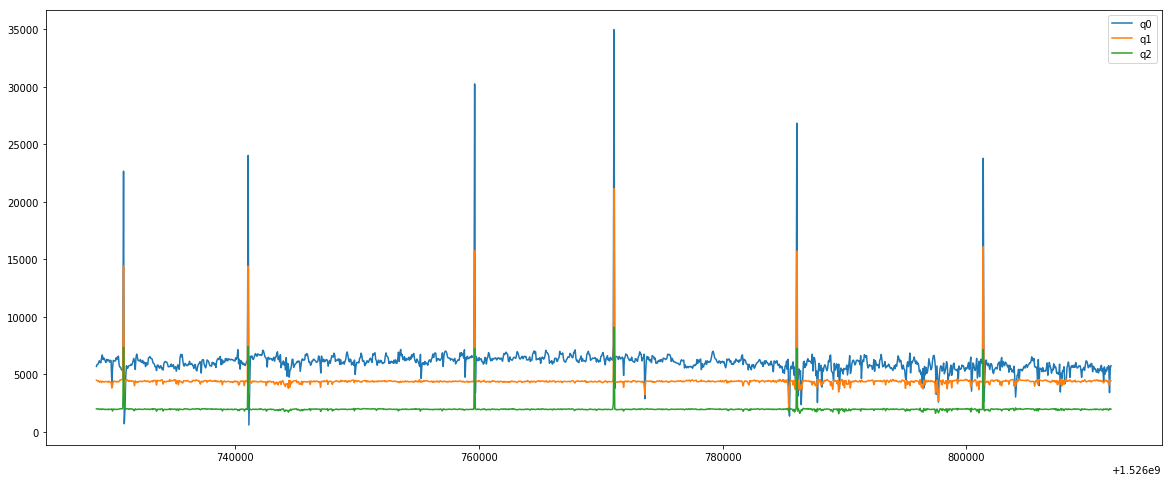
\includegraphics[width=\textwidth]{valid_cnt/valid_cnt}	
	
	\end{center}
	As convention, the blue, orange and green curves are 1-min expected messages number under QoS level respectively 0, 1 and 2.
\end{figure}

\begin{figure}
	\setlength{\tabcolsep}{0pt}
	\caption{topic: load/publish/dropped/1min}
	\label{f:valid_cnt_load_publish_dropped_1min}
	\begin{center}
	
		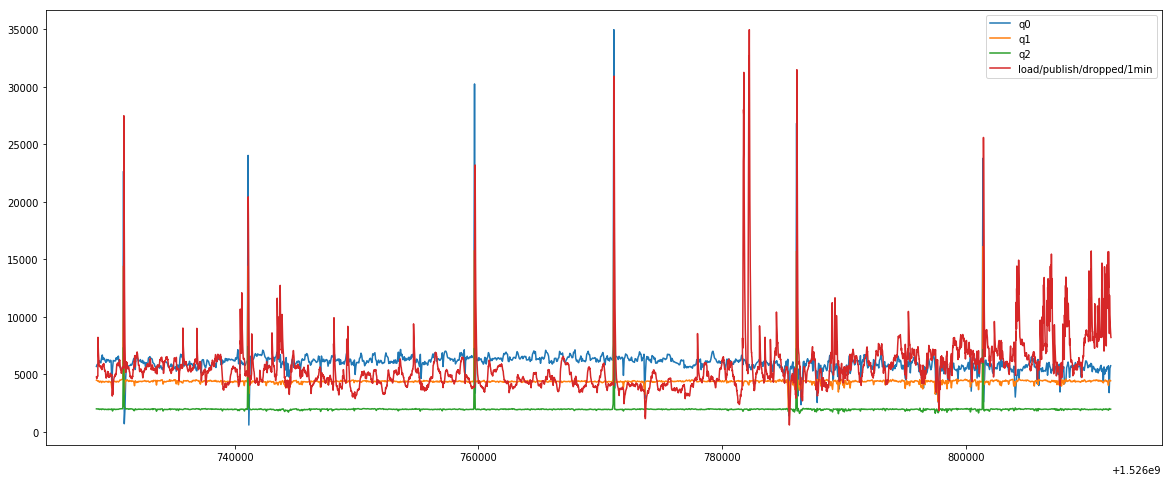
\includegraphics[width=\textwidth]{valid_cnt/valid_cnt-load_publish_dropped_1min}
	
	\end{center}
	It is observed that, surprisingly, the dropped messages largely correlates with the number of received expected messages, except for the fifth; it yet is reasonable because each peak is actually a publishing peak (shown in next figure \ref{f:valid_cnt_load_messages_sent_1min}), when the message dropping is severe as expected due to the jam.
\end{figure}

\begin{figure}
	\caption{topic: load/messages/sent/1min}
	\label{f:valid_cnt_load_messages_sent_1min}
	\begin{center}
		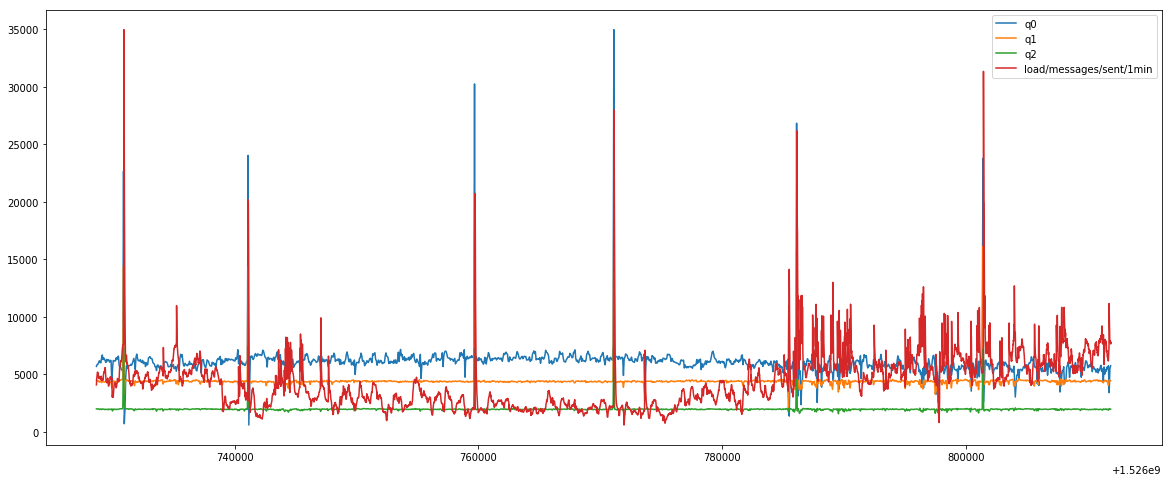
\includegraphics[width=\textwidth]{valid_cnt/valid_cnt-load_messages_sent_1min}
	\end{center}
	All the peak of 1-min expected messages number for each QoS nicely correlates with the sending peak from the SYS statics, which is expected because more it sends, more clients receive, and more chance for client to have an expected  sequential stream of received number.
\end{figure}

\begin{figure}
	\caption{topic: load/messages/received/1min}
	\label{f:valid_cnt_load_messages_received_1min}
	\begin{center}
		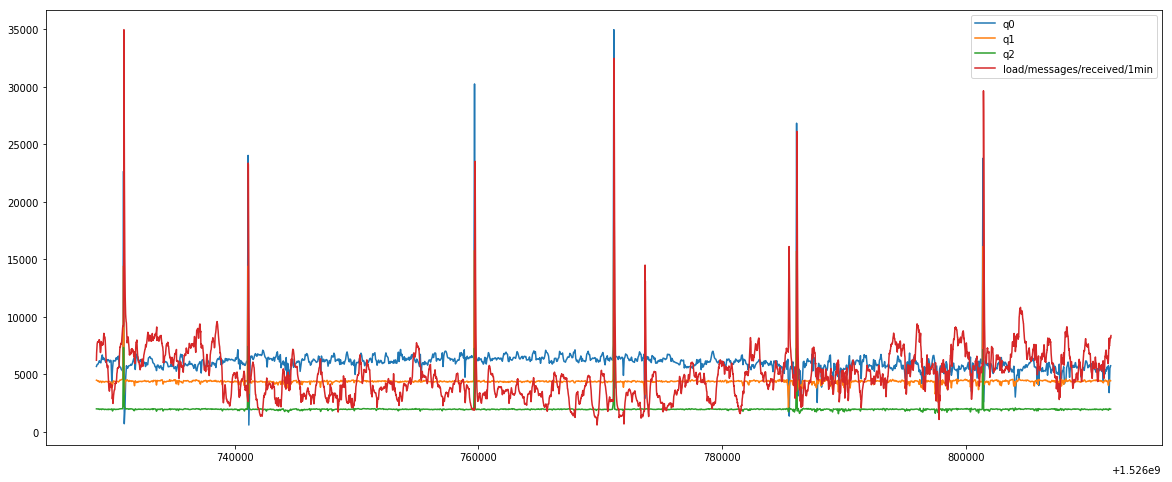
\includegraphics[width=\textwidth]{valid_cnt/valid_cnt-load_messages_received_1min}		
	\end{center}
	Again, all the peaks from SYS statics, except for some small peaks, correlates with curves for expected messages. This is expected because messages received by clients fundamentally come from the fast counter and broker needs to receives those numbers before passing them to clients.
\end{figure}

\begin{figure}
	\setlength{\tabcolsep}{0pt}
	\caption{topic: load/bytes/sent/1min}
	\label{f:valid_cnt_load_bytes_sent_1min}
	\begin{center}
		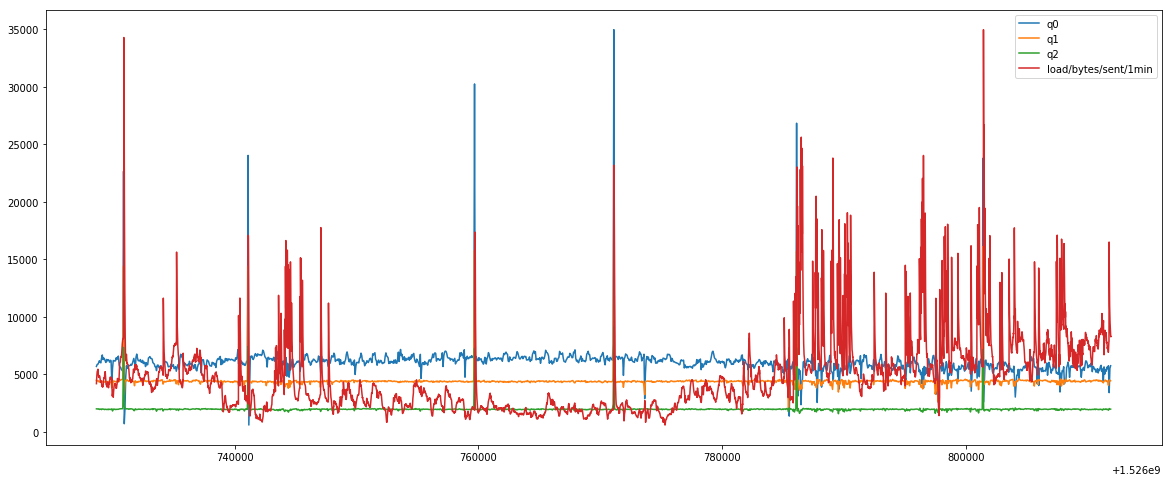
\includegraphics[width=\textwidth]{valid_cnt/valid_cnt-load_bytes_sent_1min}			
	\end{center}
	This is actually an interesting plot because it accounts for the size of each messages, where we can observe that on the left hand side around the first x-tick (740000) and after the third x-tick (780000), there are a number of small peaks of sending, denoting peaks of broker's work load for sending messages, which nicely correlates with those jitter-like peaks in previous figures (load/message/sent/1min: fig \ref{f:valid_cnt_load_messages_sent_1min}, load/publish/dropped/1min: fig \ref{f:valid_cnt_load_publish_dropped_1min}) 
\end{figure}

\begin{figure}
	\setlength{\tabcolsep}{0pt}
	\caption{topic: load/bytes/received/1min}
	\label{f:valid_cnt_load_bytes_received_1min}
	\begin{center}
		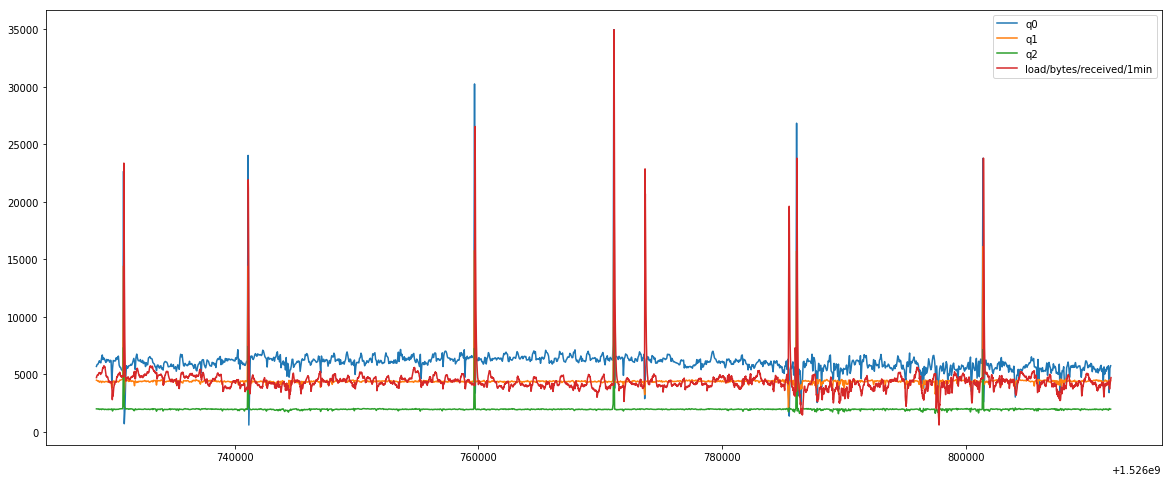
\includegraphics[width=\textwidth]{valid_cnt/valid_cnt-load_bytes_received_1min}	
	\end{center}
	It is however interesting that the messages received by the broker is not consistent with those outgoing peaks. Then why would broker suddenly needs to send bigger and more messages?
\end{figure}

\begin{figure}
	\setlength{\tabcolsep}{0pt}
	\caption{topic: load/connections/1min}
	\label{f:valid_cnt_load_connections_1min}
	\begin{center}
		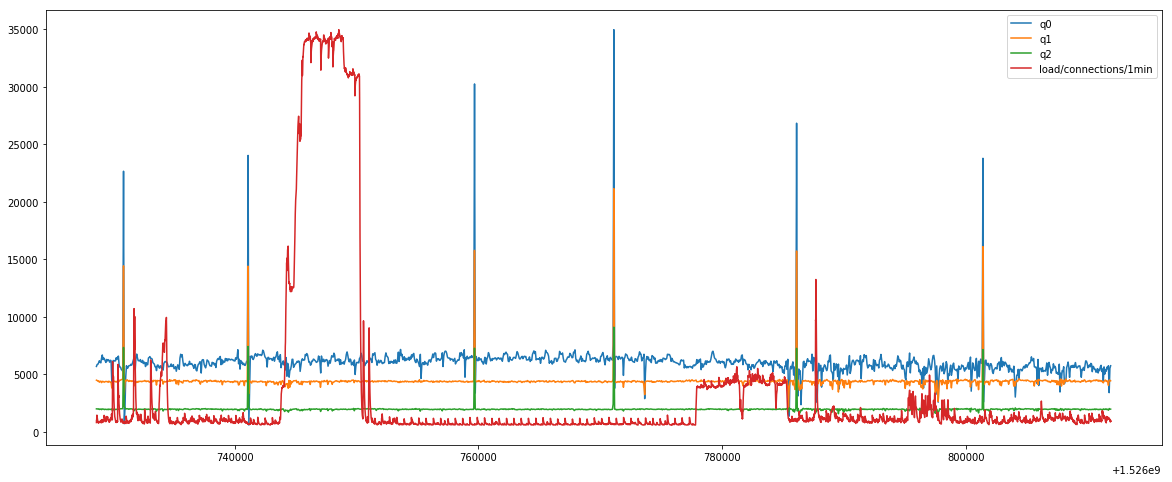
\includegraphics[width=\textwidth]{valid_cnt/valid_cnt-load_connections_1min}	
	\end{center}
	
\end{figure}

\begin{figure}
	\setlength{\tabcolsep}{0pt}
	\caption{topic: clients/connected}
	\label{f:valid_cnt_clients_connected}
	\begin{center}
		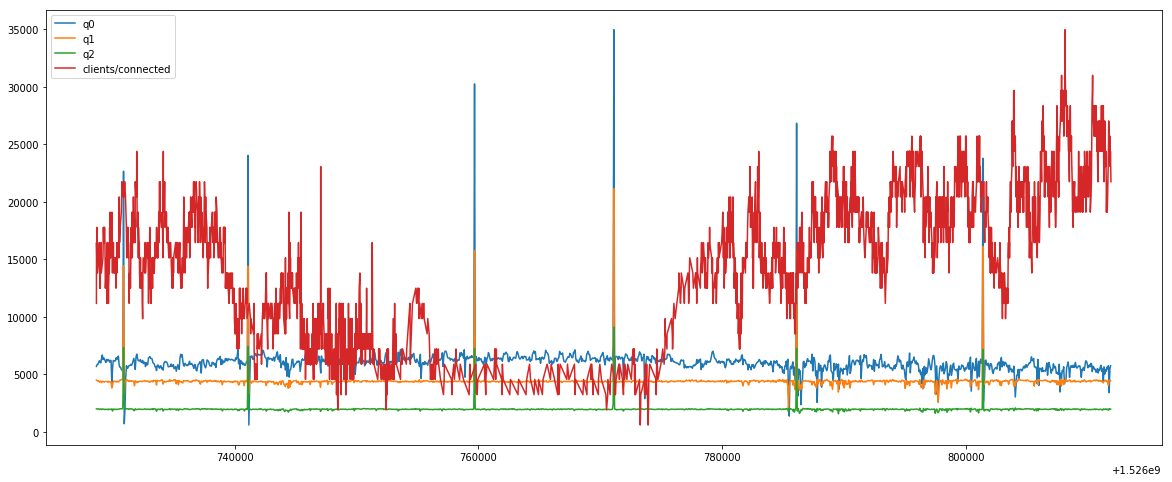
\includegraphics[width=\textwidth]{valid_cnt/valid_cnt-clients_connected}	
	\end{center}
\end{figure}

\begin{figure}
	\setlength{\tabcolsep}{0pt}
	\caption{topic: heap/current}
	\label{f:valid_cnt_heap_current}
	\begin{center}
		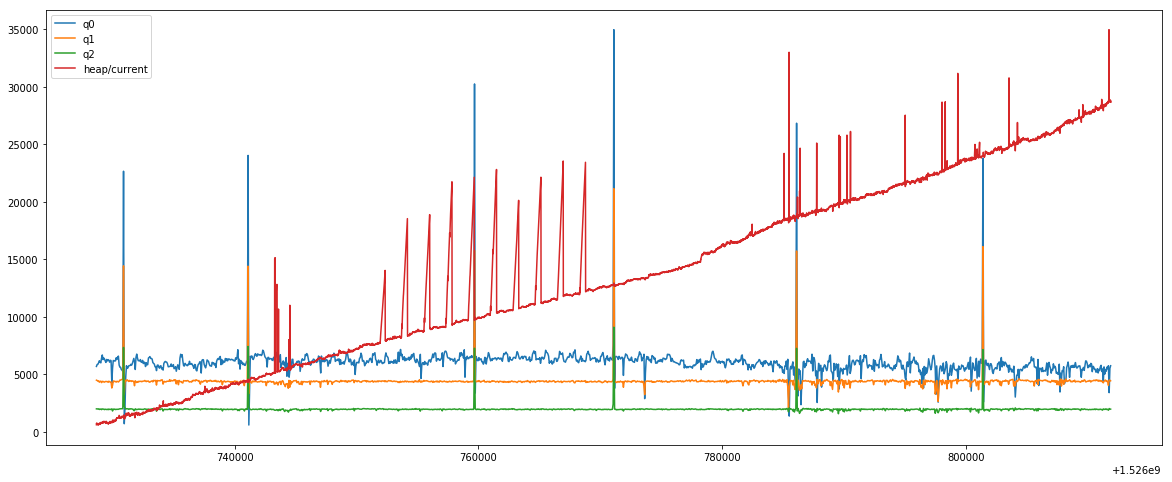
\includegraphics[width=\textwidth]{valid_cnt/valid_cnt-heap_current}	
	\end{center}
\end{figure}

\begin{figure}
	\setlength{\tabcolsep}{0pt}
	\caption{topic: heap/maximum}
	\label{f:valid_cnt_heap_maximum}
	\begin{center}
		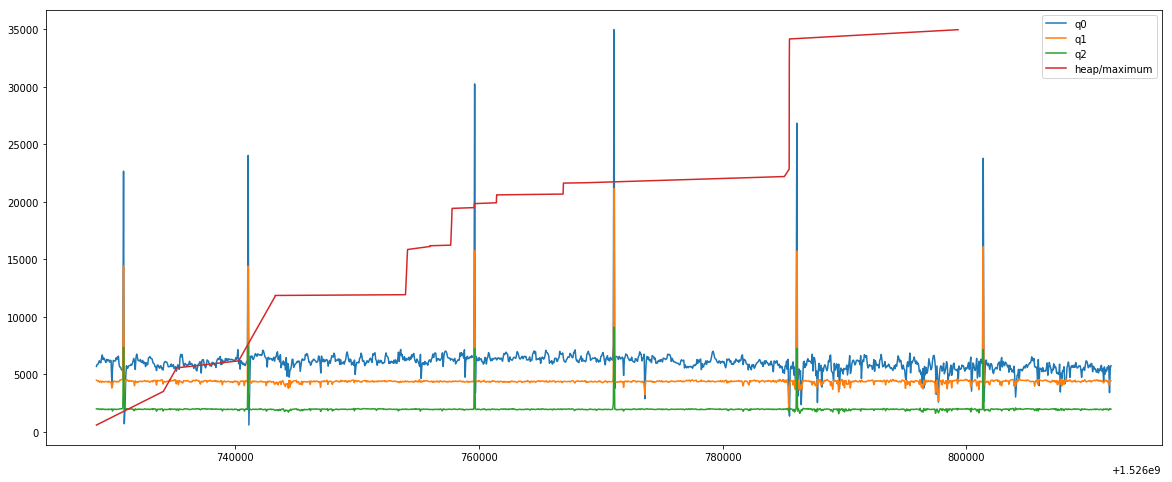
\includegraphics[width=\textwidth]{valid_cnt/valid_cnt-heap_maximum}	
	\end{center}
\end{figure}
\begin{figure}
	\setlength{\tabcolsep}{0pt}
	\caption{topic: messages/stored}
	\label{f:valid_cnt_messages_stored}
	\begin{center}
		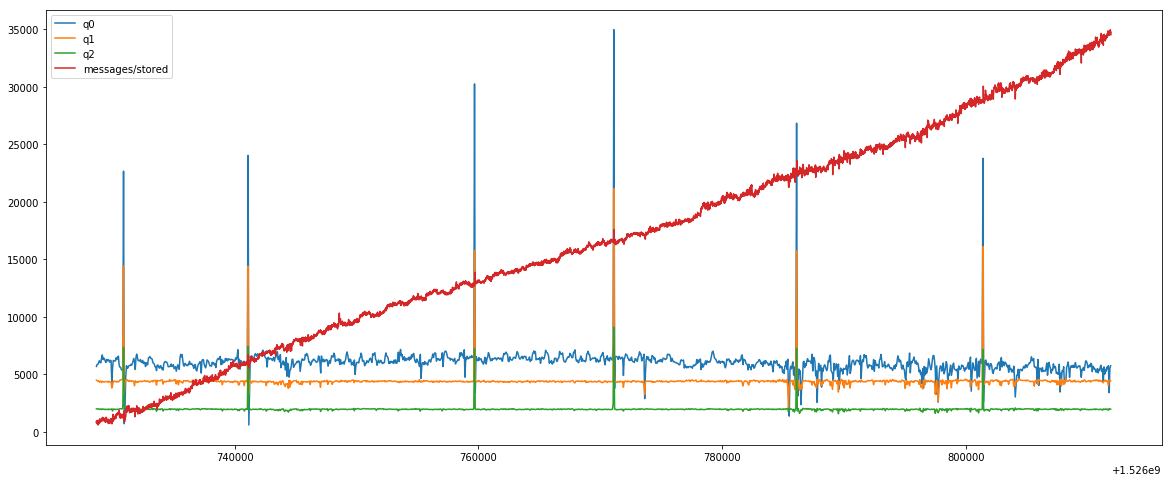
\includegraphics[width=\textwidth]{valid_cnt/valid_cnt-messages_stored}	
	\end{center}
\end{figure}
\begin{figure}
	\setlength{\tabcolsep}{0pt}
	\caption{topic: publish/messages/dropped}
	\label{f:valid_cnt_publish_messages_dropped}
	\begin{center}
		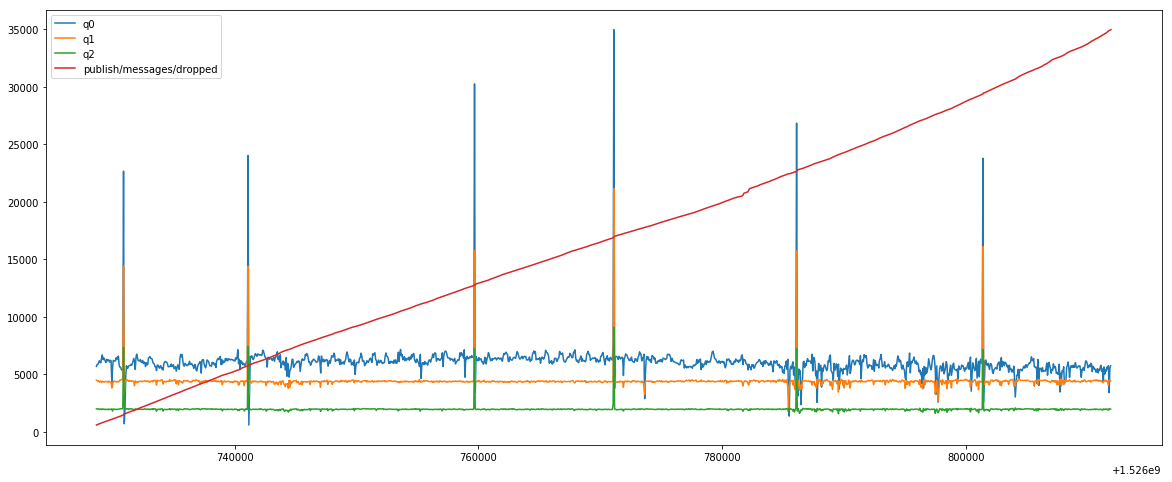
\includegraphics[width=\textwidth]{valid_cnt/valid_cnt-publish_messages_dropped}	
	\end{center}
\end{figure}
\begin{figure}
	\setlength{\tabcolsep}{0pt}
	\caption{topic: retained}
	\label{f:valid_cnt_retained}
	\begin{center}
		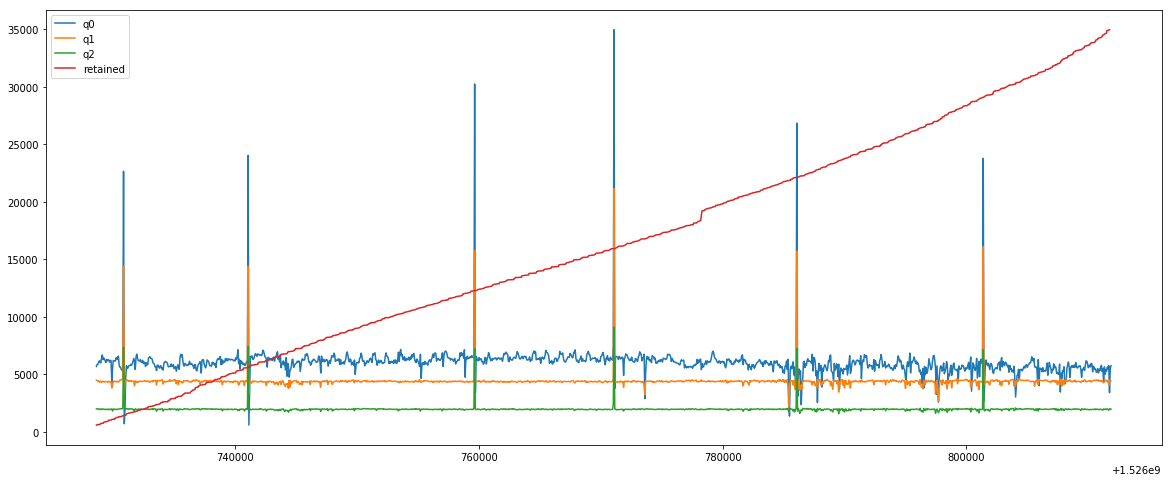
\includegraphics[width=\textwidth]{valid_cnt/valid_cnt-retained}	
	\end{center}
\end{figure}


\end{document}

